\documentclass[a4paper, 11pt]{article}
\usepackage{amsmath}
\usepackage{graphicx}
\usepackage{geometry}
\usepackage{listings}
\usepackage{float}
\usepackage{color}
\geometry{scale=0.8}
\linespread{1.5}
\usepackage{hyperref}
\definecolor{dkgreen}{rgb}{0,0.6,0}
\definecolor{gray}{rgb}{0.5,0.5,0.5}
\definecolor{mauve}{rgb}{0.58,0,0.82}
\lstset{frame=shadowbox,
    language=Prolog,
    aboveskip=3mm,
    belowskip=3mm,
    showstringspaces=false,
    columns=flexible,
    basicstyle={\small\ttfamily},
    numbers=left,
    numberstyle=\tiny\color{gray},
    keywordstyle=\color{blue},
    commentstyle=\color{dkgreen},
    stringstyle=\color{mauve},
    breaklines=true,
    breakatwhitespace=true,
    tabsize=3
}
\usepackage[colorlinks,linkcolor=red]{hyperref}

\title{	
\normalfont \normalsize
\textsc{School of Data and Computer Science, Sun Yat-sen University} \\ [25pt] %textsc small capital letters
\rule{\textwidth}{0.5pt} \\[0.4cm] % Thin top horizontal rule
\huge  E05 Family Problem ( Prolog )\\ % The assignment title
\rule{\textwidth}{2pt} \\[0.5cm] % Thick bottom horizontal rule
\author{17341203 Yixin Zhang}
\date{\normalsize\today}
}

\begin{document}
\maketitle
\tableofcontents
\newpage
\section{About Cousin and Removed}
\textbf{What Is a First Cousin, Twice Removed?}

If someone walked up to you and said, "Howdy, I'm your third cousin, twice removed," would you have any idea what they meant? Most people have a good understanding of basic relationship words such as "mother," "father," "aunt," "uncle," "brother," and "sister." But what about the relationship terms that we don't use in everyday speech? Terms like "second cousin" and "first cousin, once removed"? We don't tend to speak about our relationships in such exact terms ("cousin" seems good enough when you are introducing one person to another), so most of us aren't familiar with what these words mean.

\textbf{Relationship Terms}

Sometimes, especially when working on your family history, it's handy to know how to describe your family relationships more exactly. The definitions below should help you out.

\textbf{Cousin (a.k.a "first cousin")}

Your first cousins are the people in your family who have two of the same grandparents as you. In other words, they are the children of your aunts and uncles.

\textbf{Second Cousin}

Your second cousins are the people in your family who have the same great-grandparents as you., but not the same grandparents.

\textbf{Third, Fourth, and Fifth Cousins}

Your third cousins have the same great great grandparents, fourth cousins have the same great-great-great-grandparents, and so on.

\textbf{Removed}

When the word "removed" is used to describe a relationship, it indicates that the two people are from different generations. You and your first cousins are in the same generation (two generations younger than your grandparents), so the word "removed" is not used to describe your relationship.

The words "\textbf{once removed}" mean that there is a difference of one generation. For example, your mother's first cousin is your first cousin, once removed. This is because your mother's first cousin is one generation younger than your grandparents and you are two generations younger than your grandparents. This one-generation difference equals "once removed."

\textbf{Twice removed} means that there is a two-generation difference. You are two generations younger than a first cousin of your grandmother, so you and your grandmother's first cousin are first cousins, twice removed.
\section{Problem Description}
Please fulfill the following tasks by using \texttt{Prolog}:
\begin{enumerate}
\item Write sentences describing the predicates \textbf{Grandchild}, \textbf{Greatgrandparent}, \textbf{Ancestor}, \textbf{Brother}, \textbf{Sister}, \textbf{Daughter}, \textbf{Son}, \textbf{FirstCousin}, \textbf{BrotherInLaw}, \textbf{SisterInLaw}, \textbf{Aunt}, and \textbf{Uncle}. \emph{Hint: you can define these predicates by choosing child, sibling, male, female, father, mother, and so on. }
\item Find out the proper definition of \textbf{\emph{m}th cousin \emph{n} times removed}, in other words, define the predicate \texttt{mthCousinNremoved(X,Y,M,N)}. \emph{Hint: You'd better define the predicate \texttt{distance(X,Y,N)} by recursion ( please refer to \texttt{hanoi.pl}) to show there are N generations between X and Y in advance.}

\item Write down the basic facts depicted in the family tree in Figure \ref{fig:family}.

\item ASK it who are \textbf{Elizabeth’s grandchildren}, \textbf{Diana’s brothers-in-law}, \textbf{Zara’s great-grandparents}, and \textbf{Eugenie’s ancestors}.
\end{enumerate}

\begin{figure}[h]
  \centering
  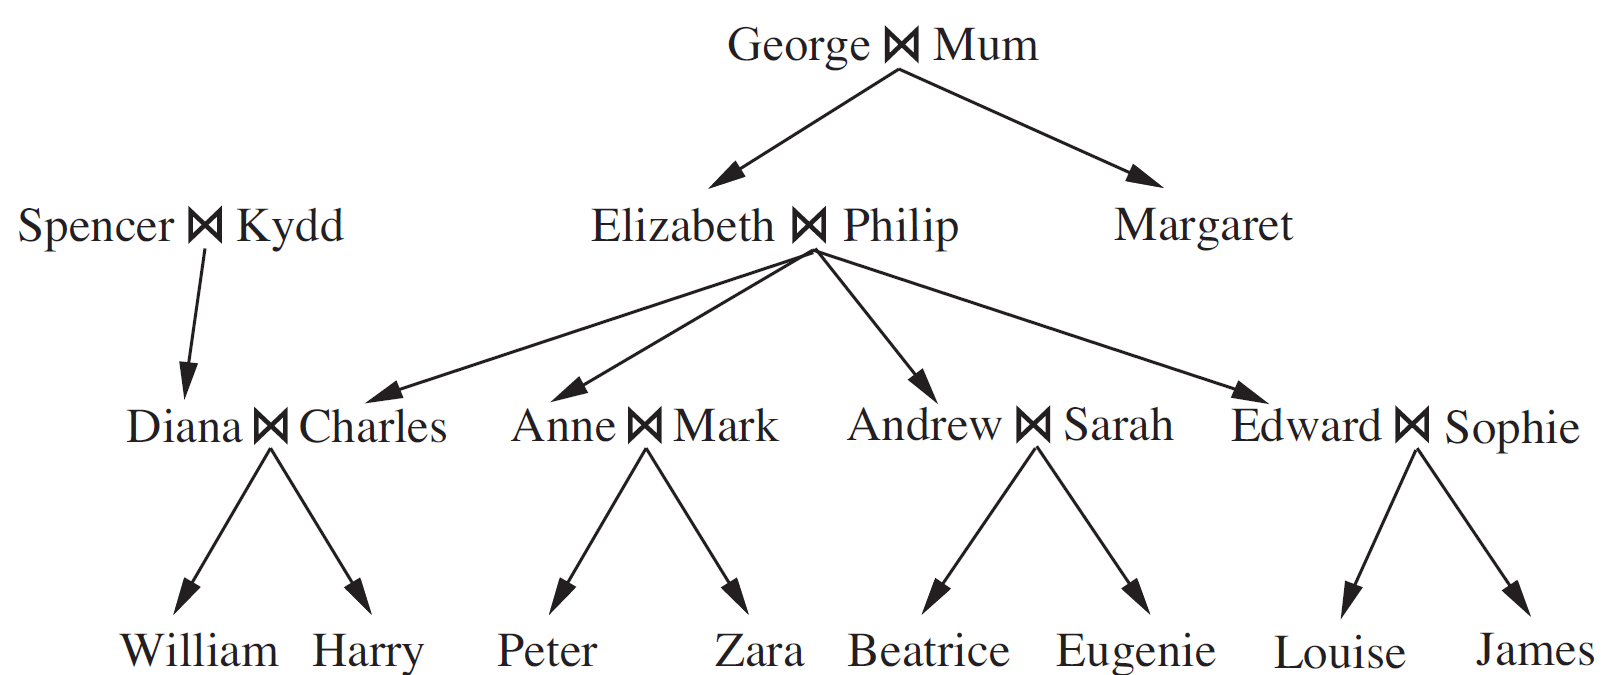
\includegraphics[width=15cm]{Pic/family}

  \label{fig:family}
  \caption{A typical family tree. The symbol $\bowtie$ connects spouses and arrows point to children.}
\end{figure}

\section{Tasks}


\begin{enumerate}
\item Please complete the \texttt{Prolog} codes. There are several tutorials in the folder and I will explain the usage of Prolog in class.
\item Write the related codes and take a screenshot of the running results in the file named \textsf{E05\_YourNumber.pdf}, and send it to \textsf{ai\_201901@foxmail.com}.

\end{enumerate}
\section{Solution}
\subsection{Overview}
I think there are two basic attributes of defining a family tree. The first thing is gender, and the second is the `child' relationship. Other relationship such as parents, siblings, grandparents, cousins can be represented by those two basic attributes.

While defining relationship between the same generation, we need to pay special attention to exclude themselves. For example, A is the first cousin of B if they have the same grandparents, and don't forget to make sure that A and B are two different persons. In Prolog, the grammer is `A$\backslash$=B'.

Another point, we need to do some work to remove duplicates. For example, when I define the `brother' relationship, I use
\begin{lstlisting}
brother(A,B):-male(A),mother(C,A),mother(C,B),A\=B.
\end{lstlisting}

instead of
\begin{lstlisting}
brother(A,B):-male(A),child(A,C),child(B,C),A\=B.
\end{lstlisting}

The latter one will consider both A's mother and A's father, thus cause duplicates.

Moreover, note that some parents are likely to have more than one children, so the relationship defined using `child' might also cause duplicates. So I define `spouse' with the following code:
\begin{lstlisting}
% define spouse relationship
husb_or_wife('George','Mum').
husb_or_wife('Spencer','Kydd').
husb_or_wife('Elizabeth','Philip').
husb_or_wife('Diana','Charles').
husb_or_wife('Anne','Mark').
husb_or_wife('Andrew','Sarah').
husb_or_wife('Edward','Sophie').
spouse(A,B):-husb_or_wife(A,B);husb_or_wife(B,A).
\end{lstlisting}

instead of the following version, which causes duplicates:
\begin{lstlisting}
spouse(A,B):-child(C,A),child(C,B),A\=B.  % this is not used because it causes dupilicates easily
\end{lstlisting}


\subsection{Code}
\begin{lstlisting}[title=family.pl]
% -- Problem 1: Predicates, expressing that "A is the xxx of B".
grandchild(A,B):-child(A,C),child(C,B).
greatGrandparent(A,B):-child(B,D),child(D,C),child(C,A).
ancestor(A,B):-child(B,A).
ancestor(A,B):-child(C,A),ancestor(C,B).
brother(A,B):-male(A),mother(C,A),mother(C,B),A\=B.   % use `mother` to remove duplicates
sister(A,B):-female(A),mother(C,A),mother(C,B),A\=B.  % use `mother` to remove duplicates
daughter(A,B):-female(A),child(A,B).
son(A,B):-male(A),child(A,B).
firstCousin(A,B):-grandchild(A,C),grandchild(B,C),A\=B.
brotherInLaw(A,B):-male(A),spouse(A,C),sister(C,B).    % sister's husband
brotherInLaw(A,B):-brother(A,C),spouse(B,C).           % husband/wife's brother
sisterInLaw(A,B):-female(A),spouse(A,C),brother(C,B).  % brother's wife
sisterInLaw(A,B):-sister(A,C),(B,C).             % husband/wife's sister
aunt(A,B):-sister(A,C),child(B,C).
aunt(A,B):-sisterInLaw(A,C),child(B,C).
uncle(A,B):-brother(A,C),child(B,C).
uncle(A,B):-brotherInLaw(A,C),child(B,C).

% some helper predicates, defined by myself
mother(A,B):-female(A),child(B,A).
father(A,B):-male(A),child(B,A).
% spouse(A,B):-child(C,A),child(C,B),A\=B.  % this is not used because it causes dupilicates easily
spouse(A,B):-husb_or_wife(A,B);husb_or_wife(B,A).
sibling(A,B):-child(A,C),child(B,C),A\=B.


% -- Problem 2: mth cousin n times removed
distance(A,A,0).
distance(C,A,K):-child(C,B),distance(B,A,K1),K is K1+1.
mthCousinNremoved(A,B,M,N):-distance(A,C,M+1),distance(B,C,M+N+1).


% -- Problem 3: Basic facts
% define gender
male('George').
male('Philip').
male('Spencer').
male('Charles').
male('Mark').
male('Andrew').
male('Edward').
male('William').
male('Harry').
male('Peter').
male('James').
female('Mum').
female('Kydd').
female('Elizabeth').
female('Margaret').
female('Diana').
female('Anne').
female('Sarah').
female('Sophie').
female('Zara').
female('Beatrice').
female('Eugenie').
female('Louise').
% define child relationship
child('Elizabeth','George').
child('Elizabeth','Mum').
child('Margaret','George').
child('Margaret','Mum').
child('Diana','Spencer').
child('Diana','Kydd').
child('Charles','Elizabeth').
child('Charles','Philip').
child('Anne','Elizabeth').
child('Anne','Philip').
child('Andrew','Elizabeth').
child('Andrew','Philip').
child('Edward','Elizabeth').
child('Edward','Philip').
child('William','Diana').
child('William','Charles').
child('Harry','Diana').
child('Harry','Charles').
child('Peter','Anne').
child('Peter','Mark').
child('Zara','Anne').
child('Zara','Mark').
child('Beatrice','Andrew').
child('Beatrice','Sarah').
child('Eugenie','Andrew').
child('Eugenie','Sarah').
child('Louise','Edward').
child('Louise','Sophie').
child('James','Edward').
child('James','Sophie').
% define spouse relationship
husb_or_wife('George','Mum').
husb_or_wife('Spencer','Kydd').
husb_or_wife('Elizabeth','Philip').
husb_or_wife('Diana','Charles').
husb_or_wife('Anne','Mark').
husb_or_wife('Andrew','Sarah').
husb_or_wife('Edward','Sophie').
\end{lstlisting}


\section{Results}
\subsection{Elizabeth's grandchildren}
\begin{figure}[H]
  \centering
  
\includegraphics[width=8cm]{Pic/1}
\end{figure}

\subsection{Diana's brothers-in-law}
\begin{figure}[H]
  \centering
  
\includegraphics[width=8cm]{Pic/2}
\end{figure}

\subsection{Zara's great-grandparents}
\begin{figure}[H]
  \centering
  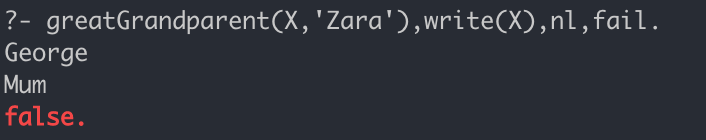
\includegraphics[width=8cm]{Pic/3}
\end{figure}

\subsection{Eugenie's ancestors}
\begin{figure}[H]
  \centering
  
\includegraphics[width=8cm]{Pic/4}
\end{figure}


%\clearpage
%\bibliography{E:/Papers/LiuLab}
%\bibliographystyle{apalike}
\end{document} 
%%% Local Variables:
%%% mode: latex
%%% TeX-master: t
%%% End:
